\epigraph{\textit{'Smack my pitch up.'}}{The Prodigy (1997)}

\section{Optimal control of pitch/travel without feedback (10.2)}

%%%%%%%%%%%%%%%%%%%%%%%%%%%%%%%%%%%%%%%%%%%%%%%%%%%%%%%%%%%%
\subsection{State space form (10.2.1)}
%%%%%%%%%%%%%%%%%%%%%%%%%%%%%%%%%%%%%%%%%%%%%%%%%%%%%%%%%%%%
We want to write the model \eqref{eq:model1} in continuous time state space form with states and input as shown in \eqref{eq:state_and_input} below.

\begin{equation}\label{eq:model1}
	\V{\dot{x}} = \M{A}_{c}\V{x} + \M{B}_{c}u
\end{equation}

\begin{equation}\label{eq:state_and_input}
\begin{aligned}
	\V{x} 	&= \begin{bmatrix}\lambda & r & p & \dot{p} \end{bmatrix}\transpose \\
	u 		&= p_{c}
\end{aligned}
\end{equation}
The equations of motion for the states are shown in \eqref{eq:state_equations} and the constants used are defined in \eqref{eq:K1K2}. (These are derived in detail in \cite{_helicopter_2015}, and will not be further explained here. The same applies for \eqref{eq:state_eqns} in section \ref{10.4.1}.) A complete table of symbols and constants lies in the appendix. 

\begin{equation}\label{eq:state_equations}
\begin{aligned}
	\dot{\lambda} 	&= r \\
	\dot{r} 		&= - K_{a} p \\
	\dot{p} 		&= \dot{p} \\
	\ddot{p} 		&= K_{1} K_{pp} (p_{c} - p) - K_{1} K_{pd} \dot{p}
\end{aligned}
\end{equation}

\begin{equation}\label{eq:K1K2}
\begin{aligned}
	K_{1} &= \frac{K_{f} l_{n}}{J_{p}} \\
	K_{2} &= \frac{K_{p} l_{a}}{J_{t}}
\end{aligned}
\end{equation}
The above gives the result in \eqref{eq:state_space_matrices}.

\begin{equation}\label{eq:state_space_matrices}
	\V{\dot{x}} =
	\underbrace{
		\begin{bmatrix}
			0 & 1 & 0 				& 0 \\
			0 & 0 & -K_{2} 			& 0 \\
			0 & 0 & 0 				& 1 \\
			0 & 0 & -K_{1}K_{pp}	& -K_{1}K_{pd}
		\end{bmatrix}
	}_{\M{A}_{c}}
	\V{x} +
	\underbrace{
		\begin{bmatrix}
			0 \\ 0 \\ 0 \\ K_{1}K_{pp}
		\end{bmatrix}
	}_{\M{B}_{c}}
	u
\end{equation}


%%%%%%%%%%%%%%%%%%%%%%%%%%%%%%%%%%%%%%%%%%%%%%%%%%%%%%%%%%%%
\subsection{Model discussion (10.2.1)}
%%%%%%%%%%%%%%%%%%%%%%%%%%%%%%%%%%%%%%%%%%%%%%%%%%%%%%%%%%%%
The system states are travel, travel rate, pitch, and pitch rate. The output of our controller is the pitch setpoint to be used by the already implemented controller, which in turn calculates voltage inputs for the hardware. We are therefore not modelling the helicopter alone, but a larger system consistinf of the helicopter along with the given controller. This corresponds with figure 7 in the exercise text \cite{_helicopter_2015}.


%%%%%%%%%%%%%%%%%%%%%%%%%%%%%%%%%%%%%%%%%%%%%%%%%%%%%%%%%%%%
\subsection{Discretisation (10.2.2)}\label{sec:disc1}
%%%%%%%%%%%%%%%%%%%%%%%%%%%%%%%%%%%%%%%%%%%%%%%%%%%%%%%%%%%%
We discretise the system by the Forward Euler Method. The general definition of the method and how it relates to our system is described by equations \eqref{eq:forward_euler} and \eqref{eq:euler_func}, respectively.

\begin{equation}\label{eq:forward_euler}
	y_{k+1} = y_{k} + h f(x_{k}, y_{k})
\end{equation}

\begin{equation}\label{eq:euler_func}
	f = \left( \M{A}_{c} \V{x}_{k} + \M{B}_c u_{k} \right)
\end{equation}
Using \eqref{eq:forward_euler} and \eqref{eq:euler_func}, we can determine the matrices of the discrete system, as shown in \eqref{eq:disc}, \eqref{eq:disc_matrix_A}, and \eqref{eq:disc_matrix_B}.

\begin{equation}\label{eq:disc}
\begin{aligned}
	\V{x}_{k+1} &= \V{x}_{k} + \left( \M{A}_{c} \V{x}_{k} + \M{B}_c u_{k} \right) h \\
				&= \V{x}_{k} + h\M{A}_{c}\V{x}_{k} + h\M{B}_{c}u_{k} \\
				&= \left( \Mc{I} + h\M{A}_{c} \right) \V{x}_{k} + h\M{B}_{c}u_{k} \\
				&= \M{A}\V{x}_{k} + \M{B}u_{k}
\end{aligned}
\end{equation}

\begin{equation}\label{eq:disc_matrix_A}
	\M{A} = \Mc{I} + h\M{A}_{c} =
	\begin{bmatrix}
		1 & h & 0 & 0 \\
		0 & 1 & -K_{2}h & 0 \\
		0 & 0 & 1 & h \\
		0 & 0 & -K_{1}K_{pp}h	& 1-K_{1}K_{pd}h
	\end{bmatrix}
\end{equation}

\begin{equation}\label{eq:disc_matrix_B}
	\M{B} = h\M{B}_c =
	\begin{bmatrix} 0 \\ 0 \\ 0 \\ K_{1}K_{pp}h \end{bmatrix}
\end{equation}


%%%%%%%%%%%%%%%%%%%%%%%%%%%%%%%%%%%%%%%%%%%%%%%%%%%%%%%%%%%%
\subsection{Discussion of the cost function (10.2.3)}
%%%%%%%%%%%%%%%%%%%%%%%%%%%%%%%%%%%%%%%%%%%%%%%%%%%%%%%%%%%%
The assignment text  \cite{_helicopter_2015} specifies a cost function \eqref{eq:cost_function} that we want to minimise subject to the constraints given in \eqref{eq:cost_constraint}.


\begin{equation} \label {eq:cost_function}
	\phi = \sum\limits_{i=1}^N (\lambda_i - \lambda_f)^2 + q p_{ci}^2, \quad q \geq 0 
\end{equation}

\begin{equation} \label{eq:cost_constraint}
	|p_k| \leq \frac{30 \pi}{180}, \quad k \in \{ 1, ..., N \}
\end{equation}

This cost function focuses on the error between $\lambda_i$ and $\lambda_f$.
It is a least-square (i.e. quadratic) function and can therefore be solved by quadratic programming methods.
The second term of the cost function involves the pitch setpoint, which is weighed by a constant $q$.


%%%%%%%%%%%%%%%%%%%%%%%%%%%%%%%%%%%%%%%%%%%%%%%%%%%%%%%%%%%%
\subsection{Procedure for solving the optimization problem (10.2.3)}
\label{optimalProcedure}
%%%%%%%%%%%%%%%%%%%%%%%%%%%%%%%%%%%%%%%%%%%%%%%%%%%%%%%%%%%%

The intention is to calculate an optimal helicopter trajectory between $x_0 = \begin{bmatrix} \lambda_0 & 0 & 0 & 0 \end{bmatrix} \transpose$ and $x_f = \begin{bmatrix} \lambda_f & 0 & 0 & 0 \end{bmatrix} \transpose$, while assuming a constant elevation angle. In this case we use $\lambda_0 = \pi$ and $\lambda_f = 0$.

We first declare the constants given in Table \ref{table:constants}, the $\M{A}$ and $\M{B}$ matrices given in \eqref{eq:state_space_matrices}, and $x_0$ given above. Then we implement the constraints in \eqref{eq:cost_constraint} using the following code:

\begin{lstlisting}
% Bounds

ul 	    = -30*pi/180;        % Lower bound on control -- u1
uu 	    = 30*pi/180;         % Upper bound on control -- u1

xl      = -Inf*ones(mx,1);   % Lower bound on states (no bound)
xu      = Inf*ones(mx,1);    % Upper bound on states (no bound)
xl(3)   = ul;                % Lower bound on state x3
xu(3)   = uu;                % Upper bound on state x3

% Generate constraints on measurements and inputs

[vlb,vub]       = genBegr2(N,M,xl,xu,ul,uu);
vlb(N*mx+M*mu)  = 0;         % We want the last input to be zero
vub(N*mx+M*mu)  = 0;         % We want the last input to be zero

\end{lstlisting}
where \texttt{genBegr2} was given on it's learning.

After that we find weight matrices for the QP problem and the matrices for the equality constrains:
\begin{lstlisting}
% Generate the matrix Q and the vector c (objecitve function weights in the QP problem) 

Q1 = zeros(mx,mx);
Q1(1,1) = 1;                	% Weight on state x1
Q1(2,2) = 0;                	% Weight on state x2
Q1(3,3) = 0;                	% Weight on state x3
Q1(4,4) = 0;                	% Weight on state x4
P1 = q;                     	% Weight on input
Q = 2*genq2(Q1,P1,N,M,mu);  	% Generate Q
c = zeros(N*mx+M*mu,1);     	% Generate c

% Generate system matrixes for linear model

Aeq = gena2(A1,B1,N,mx,mu); 	% Generate A
beq = zeros(1, size(Aeq,1));	% Generate b
beq(1:mx) = A1*x0; 	        	% Initial value
\end{lstlisting}
using \texttt{genq2} and \texttt{gena2} given on it's learning.

At last we solve the quadratic problem using the MATLAB command \texttt{quadprog}:

\begin{lstlisting}
	[z,lambda] = quadprog(Q, c, [], [], Aeq, beq, vlb, vub, z0);
\end{lstlisting}
where $\M{Z} = \begin{bmatrix} \V{x}_1 & \V{x}_2 & ... & \V{x}_N & u_1 & u_2 & ... & u_N \end{bmatrix} \transpose$. The full code is listed in the appendix. We extract the desired states and get the following plots, using three different values of $q$:


\begin{figure}[H]
        \centering
        \begin{subfigure}[b]{0.5\textwidth}
                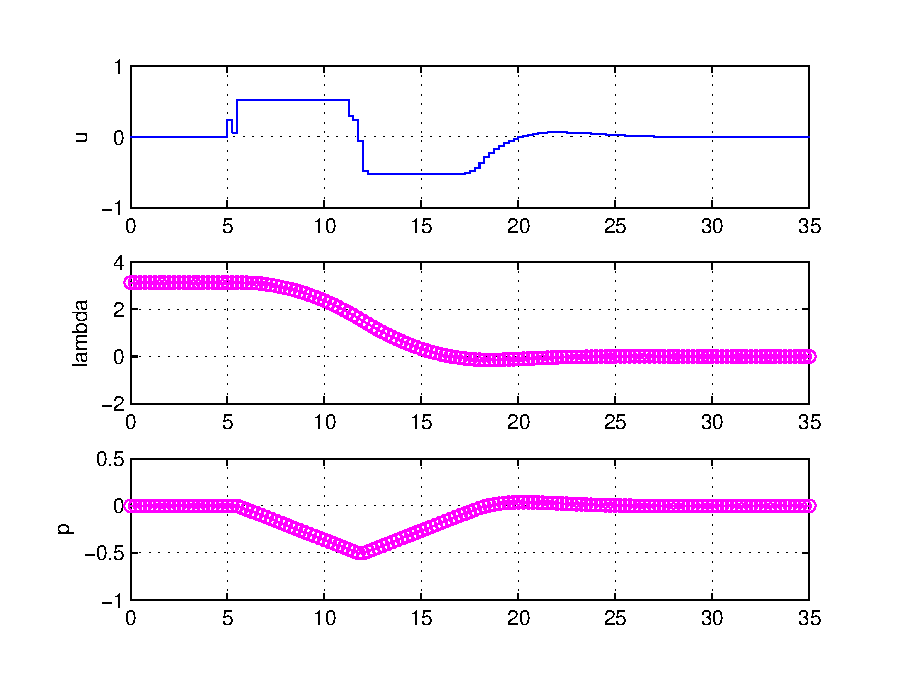
\includegraphics[width=\textwidth]{day2q0komma1}
                \caption{Optimal path with $q = 0.1$}
                \label{fig:estimatedDay201}
        \end{subfigure}%
        ~ 
        \begin{subfigure}[b]{0.5\textwidth}
                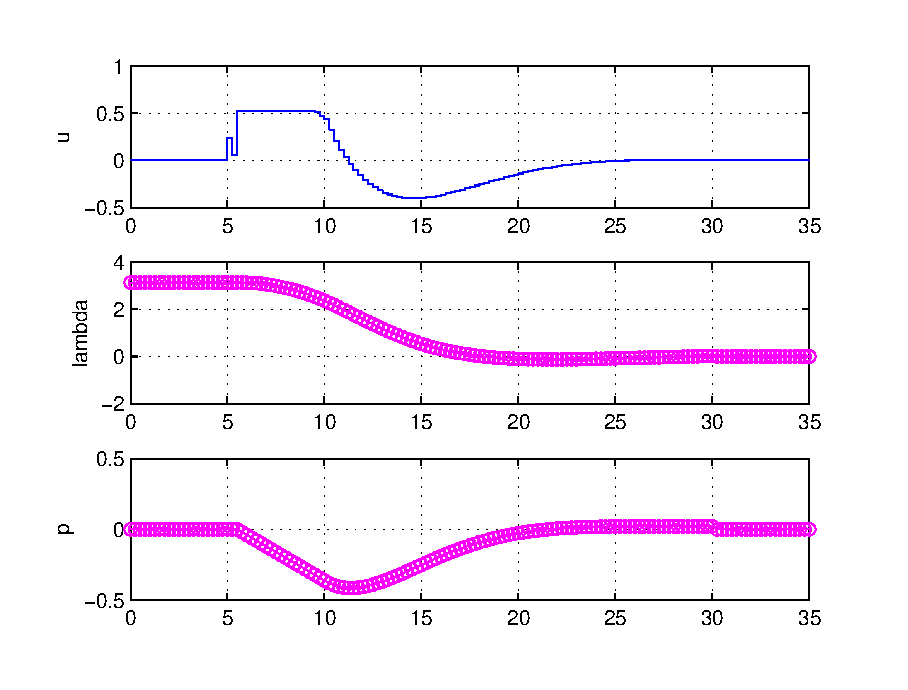
\includegraphics[width=\textwidth]{day2q1}
                \caption{Optimal path with $q = 1$}
                \label{fig:estimatedDay202}
        \end{subfigure}
        ~ 
        \begin{subfigure}[b]{0.5\textwidth}
                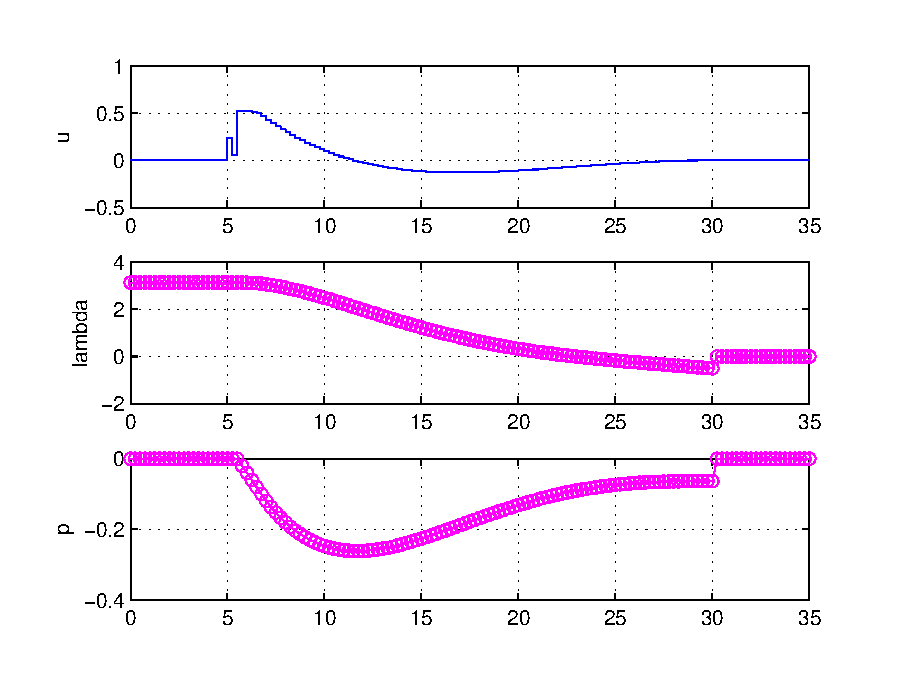
\includegraphics[width=\textwidth]{day2q10}
                \caption{Optimal path with $q = 10$}
                \label{fig:estimatedDay203}
        \end{subfigure}
        \caption{Optimal paths with different $q$}\label{fig:animals}
\end{figure}



From the figures we see that a large $q$ will downpress the pitch, resulting in slower travel. This makes sense. \eqref{eq:cost_function} tells us that $q$ is the weight of the pitch rate. We want to minimise the entire expression, meaning if we increase the weight of $p_c$, $p_c$ will decrease, to minimize the function.

%%%%%%%%%%%%%%%%%%%%%%%%%%%%%%%%%%%%%%%%%%%%%%%%%%%%%%%%%%%%
\subsection{Discussion of unwanted effects (10.2.3)\label{unwanted}}
%%%%%%%%%%%%%%%%%%%%%%%%%%%%%%%%%%%%%%%%%%%%%%%%%%%%%%%%%%%%
When $\lambda = \lambda_f$, the first part of the cost function will be 0. In this case, the QP algorithm will only attempt to minimise pitch. It achieves this by setting the pitch equal to zero, which may result in overshoot and oscillations.


%%%%%%%%%%%%%%%%%%%%%%%%%%%%%%%%%%%%%%%%%%%%%%%%%%%%%%%%%%%%
\subsection{Deviation and desired behaviour of helicopter (10.2.4)}
%%%%%%%%%%%%%%%%%%%%%%%%%%%%%%%%%%%%%%%%%%%%%%%%%%%%%%%%%%%%
Now we want to use the optimal input found in section \ref{optimalProcedure} as an input to our helicopter system. We do this using Simulink with QuaRC as seen in figure \ref{fig:heldag2}.
\begin{figure}[H]
	\centering
	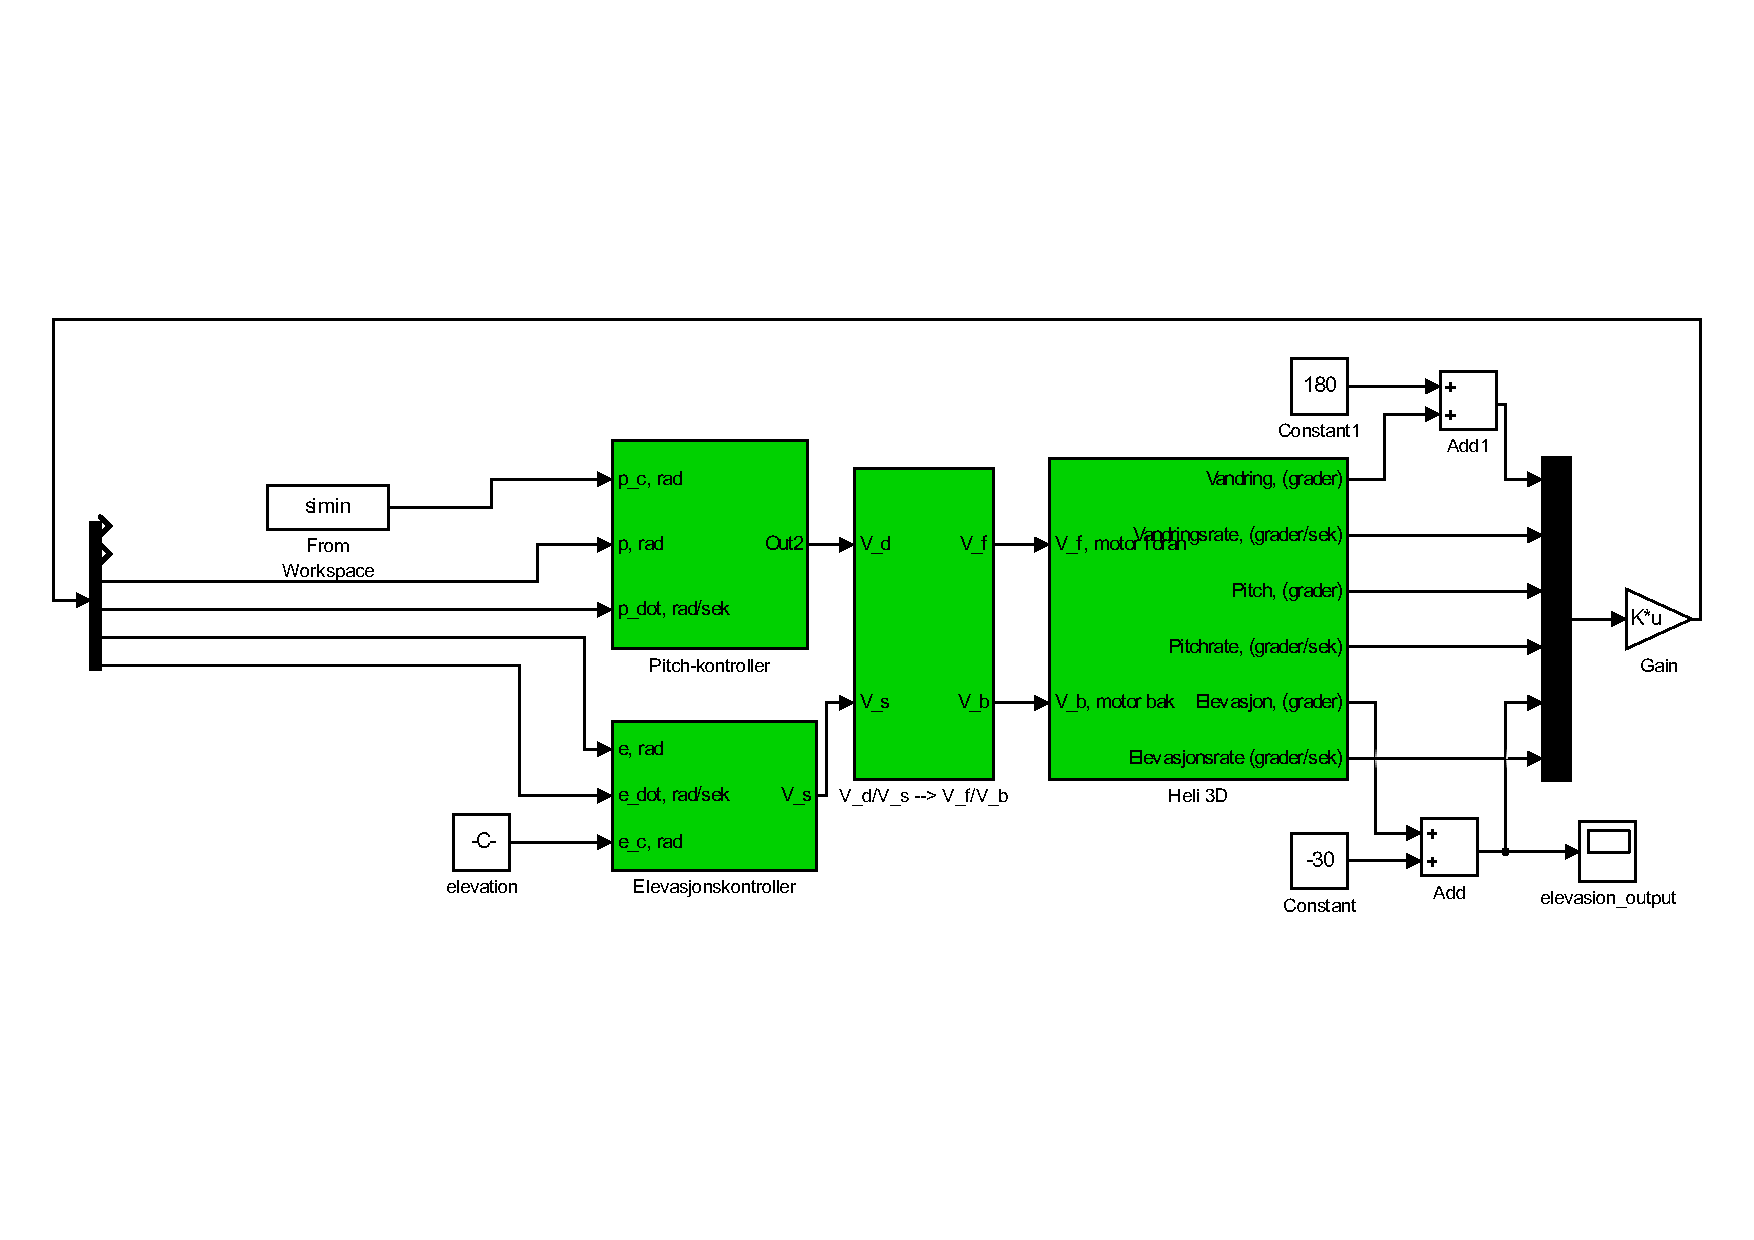
\includegraphics[width=\textwidth, trim=2cm 6cm 2cm 2cm]{simulinkmodels/heldag2}
	\caption{Simulink model of the system}
	\label{fig:heldag2}
\end{figure}

The helicopter does not stop at the desired end point, as the QP algorithm overcompensates for the time needed to brake, and the helicopter glides back in the opposite direction. This can be seen in the plots.

Note, however, that we discovered a fault related to the travel sensor causing it to not reset accumulated travel at start-up. As a consequence of this is we got a value of $\lambda$ that is off by roughly 6000 degrees, but the general response of the system is still valid and is easily seen in the figures.

\begin{figure}[H]
	\centering
	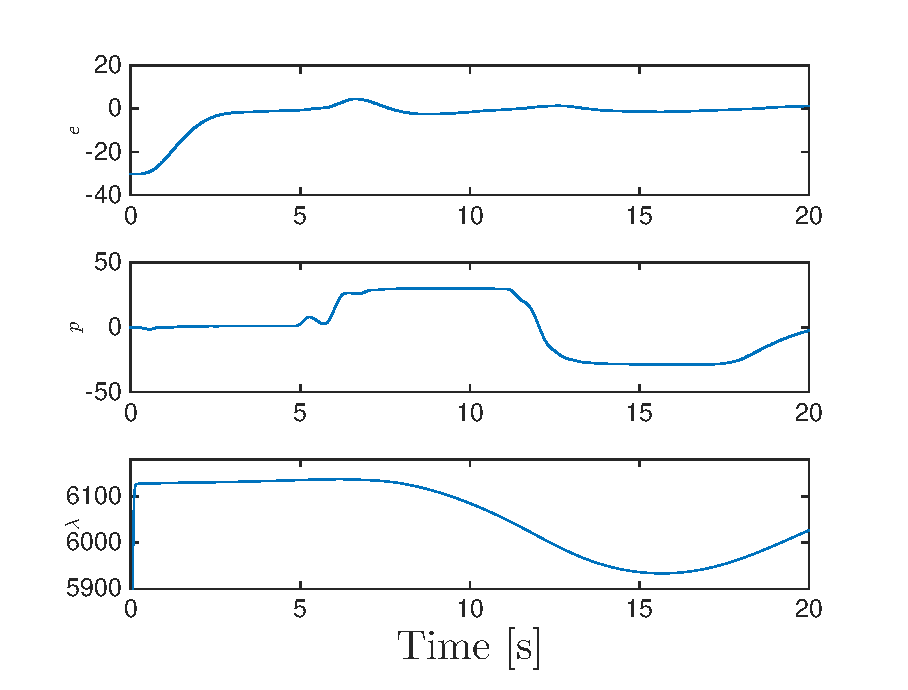
\includegraphics[width=\textwidth]{day2}
	\caption{Running the helicopter with optimal input}
	\label{fig:day2}
\end{figure}

If we compare Figure \ref{fig:day2} and Figure \ref{fig:estimatedDay202}, we see that the travel values have a similar profile for the first 15 seconds or so, after which it starts to overcompensate (as described earlier). There is some deviation of pitch, with the actual pitch first swaying one way, and then back the other. We can also see that the elevation is not constant, as opposed to our earlier assumption.